\documentclass[a4paper,9pt,twocolumn,twoside,]{pinp}

%% Some pieces required from the pandoc template
\providecommand{\tightlist}{%
  \setlength{\itemsep}{0pt}\setlength{\parskip}{0pt}}

% Use the lineno option to display guide line numbers if required.
% Note that the use of elements such as single-column equations
% may affect the guide line number alignment.

\usepackage[T1]{fontenc}
\usepackage[utf8]{inputenc}

% pinp change: the geometry package layout settings need to be set here, not in pinp.cls
\geometry{layoutsize={0.95588\paperwidth,0.98864\paperheight},%
  layouthoffset=0.02206\paperwidth, layoutvoffset=0.00568\paperheight}

\definecolor{pinpblue}{HTML}{185FAF}  % imagecolorpicker on blue for new R logo
\definecolor{pnasbluetext}{RGB}{101,0,0} %



\title{Exectutive Summary \textbar{} Boston Data Set}

\author[]{480440172, 490175477, 480561916, 480550367, 470500790}

  \affil[]{DATA2002 Group M13-07}

\setcounter{secnumdepth}{0}

% Please give the surname of the lead author for the running footer
\leadauthor{M13-07}

% Keywords are not mandatory, but authors are strongly encouraged to provide them. If provided, please include two to five keywords, separated by the pipe symbol, e.g:
 

\begin{abstract}
A city's housing is a crucial and important factor for the well-being of
residents and plays quite a significant role in the sustainability of an
economy. Rising house prices generally equate to higher rates of
\href{https://www.economicshelp.org/blog/21636/housing/how-the-housing-market-affects-the-economy/}{economic
growth} \(^{[2]}\) due to encourage consumer spending. But this can also
see first-time buyers and families struggling with increasingly
unaffordable prices in the market. This leads us to the purpose of this
investigation, which is to determine and discover what factors and
variables may be significantly impacting the median house prices. The
findings of this report suggest that factors such as crime rates, nitric
oxide concentration and several other variables do have some
statistically significant effect on the median house price in boston.
\end{abstract}

\dates{The University of Sydney 2019 Semester Two}

% initially we use doi so keep for backwards compatibility
% new name is doi_footer

\pinpfootercontents{DATA2002 M13-07}

\begin{document}

% Optional adjustment to line up main text (after abstract) of first page with line numbers, when using both lineno and twocolumn options.
% You should only change this length when you've finalised the article contents.
\verticaladjustment{-2pt}

\maketitle
\thispagestyle{firststyle}
\ifthenelse{\boolean{shortarticle}}{\ifthenelse{\boolean{singlecolumn}}{\abscontentformatted}{\abscontent}}{}

% If your first paragraph (i.e. with the \dropcap) contains a list environment (quote, quotation, theorem, definition, enumerate, itemize...), the line after the list may have some extra indentation. If this is the case, add \parshape=0 to the end of the list environment.


\hypertarget{introduction}{%
\section{Introduction}\label{introduction}}

The main purpose of this report is to explore and evaluate the factors
affecting Boston's housing prices by using multiple regression analysis.
Once a model is created and meets the assumptions, we then ask the
interesting questions to determine whether nitrious oxide concentration
and distances to Boston employment centres significantly contribute to
influencing the median value of owner-occupied homes. Housing prices can
be affected by factors such as but not limited to: location,
demographics, unemployment rates, number of rooms, etc \(^{[2]}\).
Multiple regression uses multiple predictor variables to predict an
outcome which justifies why this model can be used for the Boston
Housing dataset analysis and is therefore suitable for this analysis.

\hypertarget{the-data-set}{%
\section{The Data set}\label{the-data-set}}

To complete this investigation a dataset containing information
collected by the U.S Census Service in 1978 is used. This sample
consists of 506 entries and holds information concerning housing in the
area of Boston Mass. The dataset was obtained from StatLib archive but
was originally published by Harrison, D. and Rubinfeld, D.L.. The CSV
file used in this report was obtained from the
\href{“http://lib.stat.cmu.edu/datasets/boston”}{StatLib archive}
\(^{[3]}\) and has a total of 506 entries.

Additionally, the dataset has 14 variables which represent; crime rate
per capita, the proportion of residential land zones for lots over
25,000 square feet, the proportion of non-retail business acres, if it
was bound by a river, nitric oxides concentration, the average number of
rooms per dwelling, proportion of owner occupied units since 1940, the
distances to five Boston employment centres, the accessibility of radial
highways, the pupil teacher ratio by town, the proportion of African
Americans by town, the percentage lower status of the population and
lastly, the median value of owner-occupied homes in \$1000's.

\hypertarget{analysis}{%
\section{Analysis}\label{analysis}}

\hypertarget{model-selection-and-assumptions}{%
\subsection{Model Selection and
Assumptions}\label{model-selection-and-assumptions}}

After initial analysis of the dataset, CHAS is dropped from the data
frame, because it is a binary dummy variable that states whether a track
bounds a river, and since it is binary, it can not be used in multiple
regression. The variable MEDV is the Median value of owner-occupied
homes in \$1000's and is the variable of interest since it will assist
in establishing what affects the prices of homes. We perform a multiple
regression analysis on the variable MEDV using a backwards stepwise
procedure on a full model (Apendix). To rid of insignificant variables
we use the AIC backwards search model. After the step wise procedure,
the variables AGE and INDUS were dropped as they were proven to be
statistically insignificant to MEDV in our model.

We then decided to check the model and our assumptions, and after
viewing our residuals versus fitted plot, we decided to do a log
transformation on the model since there was a distinct pattern. Our
regression assumptions were met after our log transformation:

\begin{center}\includegraphics[width=0.95\linewidth]{assumptionSReport} \end{center}

\emph{Figure 1: Model Assumptions} \newline \newline As seen in the
residuals versus fitted plot there is no obvious patterns and therefore
it does not seem that the model has been misidentified. Regarding
homoskedasticity, the residuals don't appear to be fanning out or
changing their variability over the range of the fitted values so the
constant error variance assumption is met. in the QQ plot, the points
are reasonably close to the diagonal line, although it is possible to
argue that the points may be slightly over-dispersed. Considering that
the sample data initially contained 506 entries it is understandable to
have some deviation which is not severe enough to cause too much
concern. The normality assumption is at least approximately satisfied.
Looking at the \(R^2\) value (multiple R-squared) from the summary
output (Appendix), \textasciitilde79\% of the variability is explained
by the regression on the variables listed above. The fitted model is
seen below: \newline \newline
\(\widehat{MEDV} = 4.094 - 0.101\times\text{CRIM} + 0.001\times\text{ZN} - 0.687\times\text{NOX} + 0.092\times\text{RM} - 0.053\times\text{DIS} + 0.014\times\text{RAD} - 0.001\times\text{TAX} - 0.039\times\text{PTRATIO} + 0.001\times\text{B} - 0.029\times\text{LSTAT}\)
\newline \newline To further investigate the effect on house prices, we
may look at some variables of interest from the model. This well provide
some more explanation to our main inquiry and may also prove our model
correct.

\hypertarget{what-effect-does-dis-have-on-medv}{%
\section{What effect does DIS have on
MEDV?}\label{what-effect-does-dis-have-on-medv}}

The weighted distances to five Boston employment centres (DIS) is
significant in the model with a p-value of \(5.21 \times 10^{-12}\). In
theory this makes sense, because the closer the employment centres the
more expensive houses may be and vice versa. However, we cannot trust
the p-value without plotting the data first and determining what level
of significance DIS has on MEDV individually. \newline \newline
\textbf{Hypothesis}: \(H_0\colon\ \beta_1 = 0\) vs
\(H_1\colon\ \beta_1 \neq 0\) \newline \textbf{Assumptions}:

\begin{center}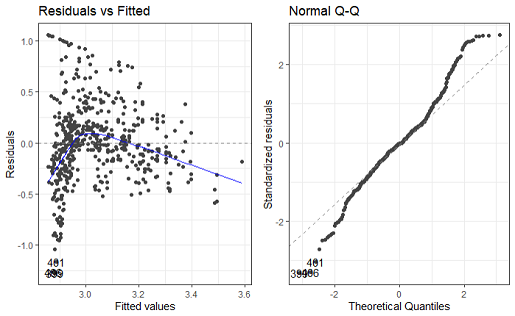
\includegraphics[width=0.95\linewidth]{inference_dis} \end{center}

\emph{Figure 2: DIS Assumptions} \newline \newline There is no
completely obvious pattern in the residual vs fitted values plot,
therefore, it does not appear that we have misspecified the model.
Regarding the homoskedasticity of the model, the residuals do not appear
to be changing their variability over the range of fitted values, and
there is no significant fanning out, therefore the constant error
variance assumption is satisfied. The QQ plot allows us to assume
normality becuase the points are reasonably close to the line. It is
important to note that there are many variables in the data set, meaning
the QQ plot will not be perfect. The normality assumption is at least
approximately satisfied.

\textbf{Test Statistic}: \(t_0 = \dfrac{1.0916}{0.1884} = 5.79\)
\newline

\textbf{P-value: }
\(2P(t_{504 }\ge 5.79) < 0.0001 (1.206612 \times 10^{-08})\) \newline

\textbf{Decision: } Since the p-value is less than 0.01 we reject the
null hypothesis and conclude that DIS does indeed have some significant
effect on house pricing. The plot for this model can be seen the
Appendix (Figure 6).

\hypertarget{what-effect-does-nox-have-on-medv}{%
\section{What effect does NOX have on
MEDV?}\label{what-effect-does-nox-have-on-medv}}

Nitric oxides concentration (NOX) may also impact house pricing, since
places with higher NOX concentrations will usually have more cars, and
therefore be more dense which most likely equate to higher house prices.
\newline

\textbf{Hypothesis}: \(H_0\colon\ \beta_1 = 0\) vs
\(H_1\colon\ \beta_1 \neq 0\) \newline

\textbf{Assumptions}:\\
All assumptions are met. Autoplot can be seen in appendix (Figure 3).
\newline

\textbf{Test Statistic}:
\(t_0 = \dfrac{-33.91606}{3.196337} = -10.61091\) \newline

\textbf{P-value: }
\(2P(t_{504 }\ge 10.61) < 0.0001 (7.065042\times10^{-24})\) \newline

\textbf{Decision: } Since the p-value is less than 0.01 we reject the
null hypothesis and conclude that NOX does indeed have some significant
effect on house pricing. The following figure displays this model:

\begin{center}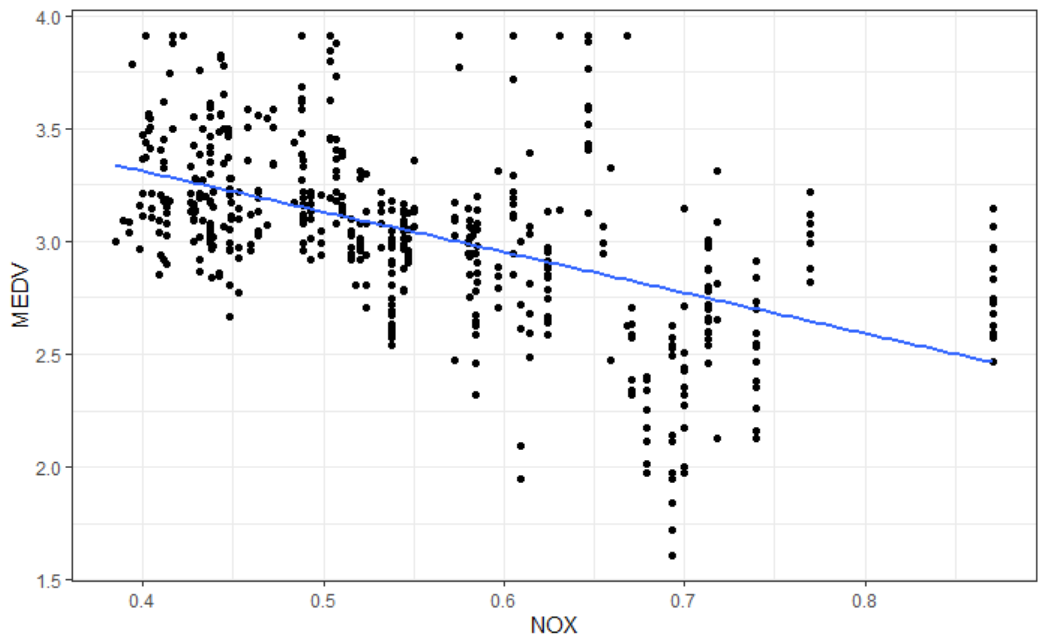
\includegraphics[width=0.95\linewidth]{nox_graph} \end{center}

\emph{Figure 4: MEDV VS NOX} \newline \newline The results are quite
interesting, becuase as NOX increases MEDV decreases, suggesting that
areas with higher Nitric oxides concentrations consist of cheaper house
than areas with less concentration.

\hypertarget{results}{%
\section{Results}\label{results}}

There is evidence that indicates a weak correlation between NOX and
Median value of the property and DIS on MEDV. Additionally, when a
linear regression is performed for them, a relatively weak linear
relationship was found for the comparisons between these 3 variables.
This was checked by obtaining the R\^{}2 values of them which were
0.2601 and 0.1157 respectively.

From the multiple regression analysis, there are 2 variables that were
found not to be significantly correlated. Namely AGE and INDUS. The
remaining 11 variables showed significant correlation with the Median
value of the properties.

\hypertarget{discussion-and-conclusion}{%
\section{Discussion and Conclusion}\label{discussion-and-conclusion}}

This report generally has many interesting findings regarding the house
market. However, despite this there are many limitations to this study
which potentially have the ability to alter and influence results. The
boston dataset used may have some issues. For instance, some of the data
was sourced from outside of Delve and may be somewhat suspect since
there is not a definite reliable source for some of the comparisons in
the dataset. Being published in 1978, it is clear the data is also quite
relatively old. This would not necessarily impact the results but may
introduce some bias to the general questions about the median house
market in today's society. In a future analysis, it would defenifenity
be more appropriate to investigate a data set that is recent and
reliable to ensure contemporary and relevant results. In addition to
this, there is some evident departure on the QQ plot and there is a
small pattern of over-fitting, however, the dataset is quite large and
this is somewhat expected when dealing with larger datasets. Despite
this, perhaps in future investigations it will be more fitting to have a
deeper analysis into the variables and a wider range of model selection.

In conclusion, from our multiple regression, we found that housing
prices in Boston is found to be not significantly correlated with (AGE)
and proportion of non-retail business acres per town (INDUS). This model
was reasonably accurate in predicting median house prices
(\(R^2 = 0.79\)). The linear models show that nitrious oxide levels and
distance to employment centres are a relatively weak direct
relationship, so we can assume that it does play somewhat of a role in
influencing housing price. \newline \newline

\hypertarget{references}{%
\section{References}\label{references}}

{[}1{]} Harrison, D, and D.L Rubinfeld. ``Hedonic Prices and the Demand
for Clean Air.'' J. Environ. Economics \& Management, StatLib archive ,
10 Oct.~1996, lib.stat.cmu.edu/datasets/boston \newline
[2] Pettinger, Tejvan. ``How the Housing Market Affects the Economy.''
Economics Help, EconomicsHelp.org, 24 Apr.~2019,
www.economicshelp.org/blog/21636/housing/how-the-housing-market-affects-the-economy/.
\newline
[3] Data Set Source: \url{http://lib.stat.cmu.edu/datasets/boston}

\hypertarget{appendix}{%
\section{Appendix}\label{appendix}}

\begin{center}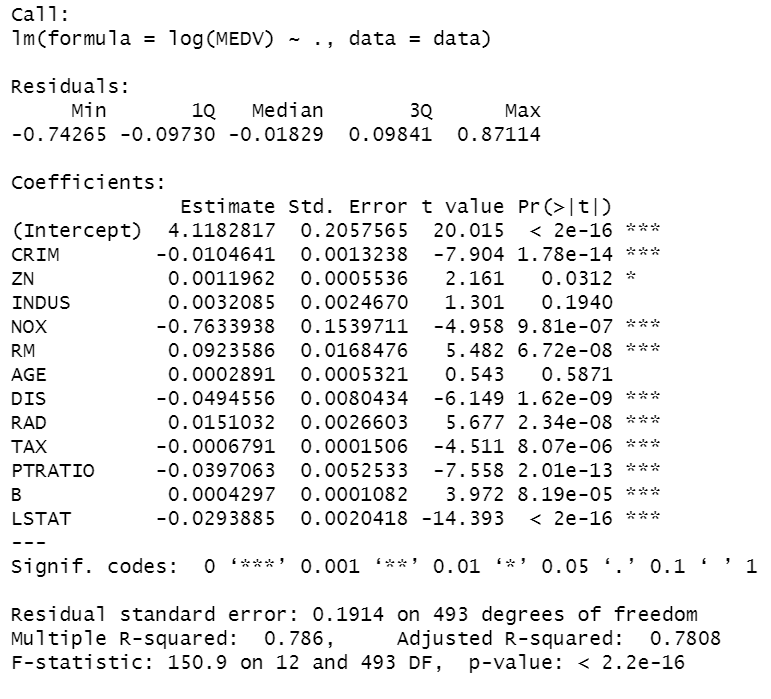
\includegraphics[width=0.95\linewidth]{full} \end{center}

\emph{Figure 7: Full Model} \newline

\begin{center}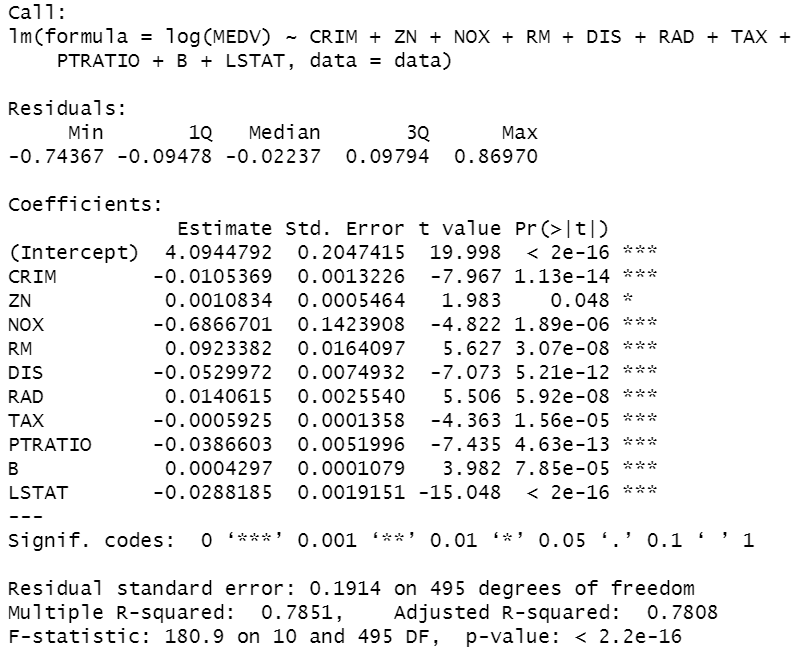
\includegraphics[width=0.95\linewidth]{dropped} \end{center}

\emph{Figure 8: Model with dropped AGE and INDUS} \newline \newline
\newline \newline \newline

\begin{center}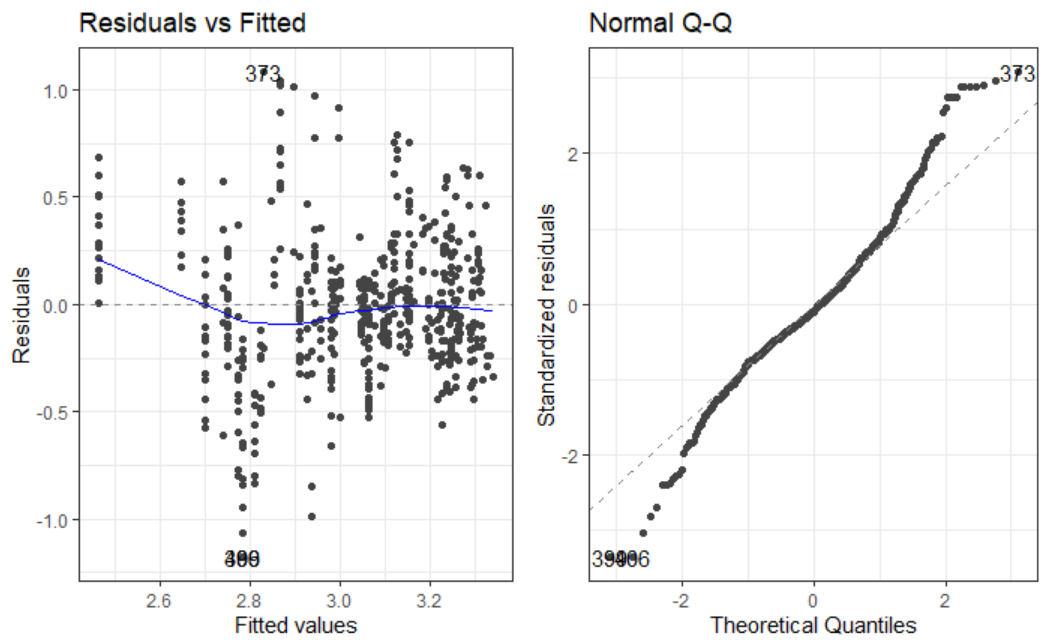
\includegraphics[width=0.95\linewidth]{nox_ass} \end{center}

\emph{Figure 3: NOX Assumptions} \newline

\begin{center}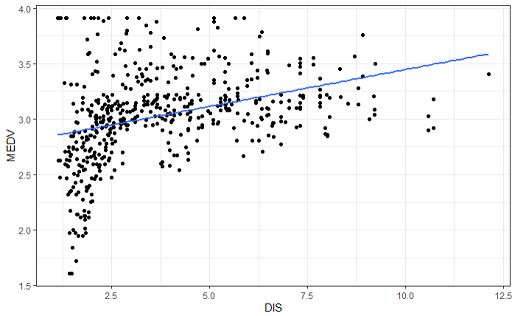
\includegraphics[width=0.95\linewidth]{inference_dis_graph} \end{center}

\emph{Figure 6: DIS VS MEDV} \newline

%\showmatmethods


\bibliography{pinp}
\bibliographystyle{jss}



\end{document}

